%
% IEEE Transactions on Microwave Theory and Techniques example
% Tibault Reveyrand - http://www.microwave.fr
%
% http://www.microwave.fr/LaTeX.html
% ---------------------------------------



% ================================================
% Please HIGHLIGHT the new inputs such like this :
% Text :
%  \hl{comment}
% Aligned Eq. 
% \begin{shaded}
% \end{shaded}
% ================================================



\documentclass[journal]{IEEEtran}

%\usepackage[retainorgcmds]{IEEEtrantools}
%\usepackage{bibentry}  
\usepackage{xcolor,soul,framed} %,caption

\colorlet{shadecolor}{yellow}
% \usepackage{color,soul}
\usepackage[pdftex]{graphicx}
\graphicspath{{../pdf/}{../jpeg/}}
\DeclareGraphicsExtensions{.pdf,.jpeg,.png}

\usepackage[cmex10]{amsmath}
%Mathabx do not work on ScribTex => Removed
%\usepackage{mathabx}
\usepackage{array}
\usepackage{mdwmath}
\usepackage{mdwtab}
\usepackage{eqparbox}
\usepackage{url}

\hyphenation{op-tical net-works semi-conduc-tor}

%\bstctlcite{IEEE:BSTcontrol}


%=== TITLE & AUTHORS ====================================================================
\begin{document}
\bstctlcite{IEEEexample:BSTcontrol}
    \title{Paper title}
  \author{
  Ibrahim Khalid,
      Justin Wang,
      Shrey Agarwal,
      Harsh Shinde,
      Ashwini Hiremath
      }



% The paper headers
\markboth{paper header, do we need this?}{paper header, do we need this?}


\maketitle



\begin{abstract}
Project abstract here
\end{abstract}

\begin{IEEEkeywords}
Keywords, here
\end{IEEEkeywords}


\IEEEpeerreviewmaketitle

% === I. INTRODUCTION =============================================================
% =================================================================================
\section{Introduction}

\IEEEPARstart{T}{he} first sentence starts with a big letter

\section{Section Header}


\begin{figure}[!htb]
  \begin{center}
  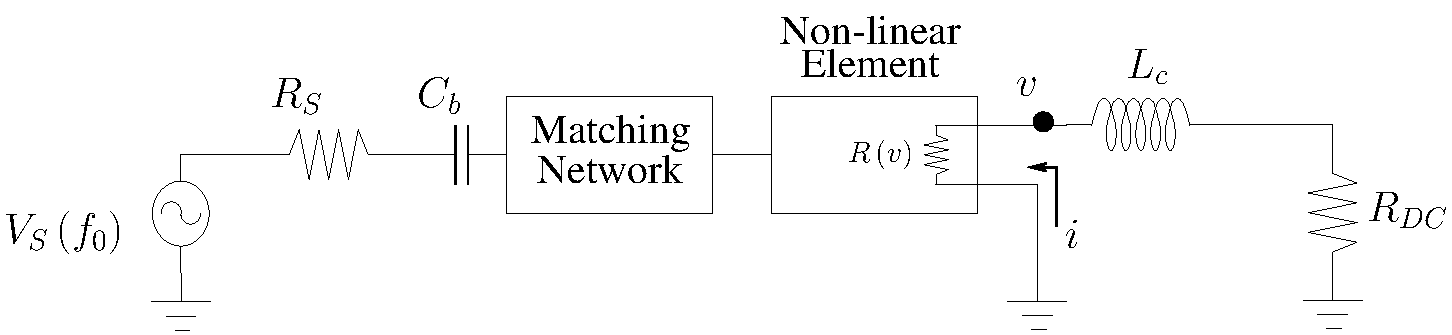
\includegraphics[width=3.5in]{pdf/01.pdf}\\
  \caption{This is how to add a figure and caption}
  \label{circuit_diagram}
  \end{center}
\end{figure}

This is how to reference a Fig.~\ref{circuit_diagram}.

This is how to write an equation and reference it like eq. \ref{ideal_rectifier_resistance}.
\begin{equation}
\label{ideal_rectifier_resistance}
R(v) =
\begin{cases}
    \infty, & v > 0\\
    0, & v \leq 0
\end{cases}
\end{equation}

\subsection {Subsection header}

\begin{itemize}
    \item This
    \item is
    \item how to make an unnumbered list
\end{itemize}


\begin{enumerate}
    \item This
    \item is
    \item how to make a numbered list
\end{enumerate}


\section{Conclusion}
This is how to cite something \cite{brown}


\section*{Acknowledgment}
Do we need this section?



\ifCLASSOPTIONcaptionsoff
  \newpage
\fi


\bibliographystyle{IEEEtran}
\bibliography{IEEEabrv,Bibliography}

\begin{IEEEbiography}[{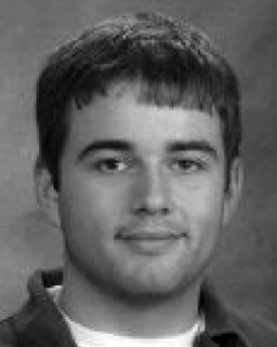
\includegraphics[width=1in,height=1.25in,clip,keepaspectratio]{photo/mike.png}}]{Michael Roberg}
Do we need a bio section? We should ask the professor
\end{IEEEbiography}
\vfill
\end{document}